\documentclass[12pt,a4paper]{report}

% Packages for fonts and formatting
\usepackage{mathptmx} % Times New Roman
\usepackage[margin=1in]{geometry}
\usepackage{setspace}
\onehalfspacing

% Packages for structure and styling
\usepackage{titlesec}
\usepackage{cite}
\usepackage{hyperref}
\usepackage{tikz}
\usetikzlibrary{shapes.geometric, arrows}
\usepackage{etoolbox}
\usepackage{enumitem}

\makeatletter
\patchcmd{\chapter}{\if@openright\cleardoublepage\else\clearpage\fi}{}{}{}
\patchcmd{\chapter}{\clearpage}{}{}{}
\makeatother

\setlist{itemsep=0.3em, topsep=0.3em, parsep=0.1em}

\hypersetup{
    colorlinks=true,
    linkcolor=black,
    filecolor=black,      
    urlcolor=black,
    citecolor=black,
}

% Redefine chapter and section formatting to make it more compact and professional
\titleformat{\chapter}[block]
  {\normalfont\huge\bfseries}{\thechapter.}{1em}{}
\titlespacing*{\chapter}{0pt}{20pt}{15pt}
\titlespacing*{\section}{0pt}{10pt}{5pt}

\begin{document}

\begin{titlepage}
    \begin{center}
        \vspace*{1cm}
        
        \Huge
        \textbf{Medical Specialty Classification using TF-IDF and Ensemble Machine Learning}
        
        \vspace{1.5cm}
        
        \Large
        \textbf{Mini Project Proposal Report}
        
        \vspace{2.5cm}
        
        \large
        \textbf{Submitted by:} \\
        Jiphin George \\
        Register No.: MAC25MCA-2033
        
        \vspace{1.5cm}
        
        \textbf{Submitted to:} \\
        Prof. Biju Skaria \\
        Project Guide
    \end{center}
    
    \vfill
    
    \begin{center}
        \Large
        \textbf{Department of Computer Applications}
        
        \vspace{0.5cm}
        
        \textbf{Mar Athanasius College of Engineering} \\
        Kothamangalam, Kerala
        
        \vspace{0.5cm}
        
        \large
        \textbf{Master of Computer Applications (MCA)}
        
        \vspace{0.5cm}
        
        Academic Year: 2026--2027
        \vspace*{1cm}
    \end{center}
\end{titlepage}

\chapter{Introduction}
The adoption of Electronic Health Records (EHRs) has grown exponentially over the past decade, resulting in a massive digitization of patient data across global healthcare networks. While structured data points like vital signs are easily managed, the vast majority of clinical information is captured as unstructured text in the form of medical transcriptions, physician notes, and discharge summaries. The increasing volume of this unstructured clinical text presents a critical bottleneck for hospital administrators who must efficiently process, categorize, and route these documents to specialized departments. Natural Language Processing (NLP) has emerged as an indispensable technology in this domain, providing the computational tools necessary to automate the analysis of complex medical narratives. By bridging the gap between human language and machine understanding, NLP enables the automated classification of these documents, naturally transitioning medical informatics from slow, manual sorting to intelligent, algorithm-driven routing systems.

\section{Background}
The rapid digitization of global healthcare systems has resulted in the unprecedented accumulation of clinical data. Electronic Health Records (EHRs) and medical transcriptions encompass comprehensive patient histories, diagnoses, and treatment plans. However, a significant portion of this invaluable clinical documentation is stored in unstructured, narrative text formats. Medical transcription, the process of converting voice-recorded medical reports dictated by healthcare practitioners into text, generates vast quantities of data. Traditionally, these transcription reports are manually reviewed and organized by specific medical specialties, such as Cardiology, Neurology, or Orthopedics. 

\section{Motivation}
The primary motivation for this project is to address the severe inefficiencies associated with the manual handling of healthcare documents. As patient populations and data volumes grow exponentially, manual classification methods become unsustainable. Automating this process using Natural Language Processing (NLP) and Machine Learning (ML) can effectively reduce administrative overhead, ensure consistent document routing, and allow healthcare professionals to redirect their focus from clerical tasks directly to patient care. To improve classification robustness and reduce the limitations of relying on a single classifier, this project proposes a Voting Ensemble approach that combines multiple machine learning models.

\section{Problem Statement}
In contemporary healthcare institutions, organizing unstructured medical documents remains a substantial administrative challenge. Relying on manual categorization by hospital personnel is inherently slow, financially expensive, and subject to natural human error. The subjective interpretation of complex medical jargon frequently leads to inconsistent categorizations, which can misroute critical patient information and severely delay clinical workflows. Therefore, the core problem is the lack of an efficient, scalable, and highly accurate automated mechanism capable of classifying unstructured clinical text into precise medical specialties.

\par
\chapter{Objectives}
The primary objective of the proposed project is to design, develop, and evaluate an automated machine learning system capable of accurately classifying medical transcription reports into their respective medical specialties. Specifically, the project aims to:
\begin{itemize}
    \item Implement a robust Natural Language Processing preprocessing pipeline to clean and standardize noisy clinical text.
    \item Extract highly discriminative numerical features from unstructured medical narratives using Term Frequency-Inverse Document Frequency (TF-IDF).
    \item Train and evaluate multiple baseline machine learning algorithms (Logistic Regression, Support Vector Machine, Random Forest, Multinomial Naïve Bayes) on the clinical dataset.
    \item Develop a Voting Ensemble Classifier that combines the predictive strengths of the individual base models to maximize overall classification accuracy and robustness.
    \item Deploy the finalized ensemble model through a lightweight, user-friendly Flask web application to demonstrate real-world clinical applicability.
    \item Compare the performance of the individual machine learning models with the Voting Ensemble Classifier to identify the most effective approach for medical specialty classification.
\end{itemize}

\par
\chapter{Proposed Methodology}
The proposed project will follow a structured, sequential methodology to transform raw medical text into accurate specialty predictions.

\section{Dataset}
The system will utilize the Medical Transcriptions (MTSamples) dataset. This publicly available corpus contains around 5,000 medical transcription reports spanning various clinical specialties. It appropriately exemplifies the complexities and imbalances inherent in real-world clinical documentation. The dataset consists of unstructured clinical narratives dictated by healthcare professionals, covering diverse medical domains such as Surgery, Cardiology, and Neurology. Because it accurately mirrors the linguistic structure of actual patient records, it is highly suitable for evaluating traditional NLP and machine learning approaches.

\section{Data Preprocessing}
Recognizing that raw clinical text cannot be directly ingested by mathematical models, a rigorous preprocessing pipeline will be executed:
\begin{itemize}
    \item \textbf{Lowercasing:} Converting all text to lowercase to ensure uniform mathematical treatment of words regardless of capitalization.
    \item \textbf{Tokenization:} Fracturing continuous clinical narratives into discrete word units (tokens) using NLP libraries.
    \item \textbf{Stop-word removal:} Systematically filtering out common, non-informative English vocabulary that dilutes the predictive power of the dataset.
    \item \textbf{Lemmatization:} Reducing all remaining clinical tokens to their absolute linguistic root forms (e.g., converting ``operating'' and ``operated'' to ``operate'').
\end{itemize}

\section{TF-IDF Feature Extraction}
Following preprocessing, the system will systematically apply Term Frequency-Inverse Document Frequency (TF-IDF) vectorization. This statistical technique will evaluate the entire clinical corpus to generate high-dimensional numerical feature vectors. TF-IDF explicitly highlights unique, highly discriminative medical terminology specific to particular specialties while mathematically suppressing ubiquitous words, appropriately structuring the data for algorithmic ingestion.

\section{Machine Learning Models}
The core computational engine will independently train four traditional machine learning classifiers on the extracted TF-IDF feature space:
\begin{itemize}
    \item \textbf{Logistic Regression:} A robust linear model highly effective for high-dimensional text classification.
    \item \textbf{Support Vector Machine (SVM):} An algorithm that attempts to find the optimal mathematical hyperplane to separate different medical specialty classes.
    \item \textbf{Random Forest:} A tree-based ensemble method that reduces overfitting by averaging multiple decision trees.
    \item \textbf{Multinomial Naïve Bayes:} A probabilistic classifier particularly suited for word frequency features.
\end{itemize}

\section{Voting Ensemble Classifier}
Building upon the independently trained baselines, a Hard Voting Ensemble Classifier will be developed. This architecture will effectively combine the multiple classifiers into a unified predictive system. By aggregating the discrete class predictions of the individual models and calculating the absolute statistical majority, the ensemble framework will mathematically mitigate individual algorithmic biases, yielding a significantly more stable and accurate final prediction.

\section{Flask Web Application}
To ensure practical accessibility, a responsive web interface will be constructed utilizing HTML, CSS, and the lightweight Python Flask framework. The serialized ensemble model and TF-IDF vectorizers will be integrated into the backend, allowing users to efficiently input raw medical text and instantly receive the predicted medical specialty.

\section{Evaluation Strategy}
The system will be subjected to rigorous statistical evaluation using an unseen testing dataset. Performance will be quantified using standard classification metrics:
\begin{itemize}
    \item \textbf{Accuracy:} The overall percentage of correctly classified reports.
    \item \textbf{Precision:} The proportion of true positive predictions among all positive predictions for a given specialty.
    \item \textbf{Recall:} The proportion of true positive predictions among all actual instances of a given specialty.
    \item \textbf{F1-score:} The harmonic mean of Precision and Recall, crucial for evaluating performance on the imbalanced MTSamples dataset.
\end{itemize}

\section{Proposed Workflow}

\begin{figure}[htbp]
\centering
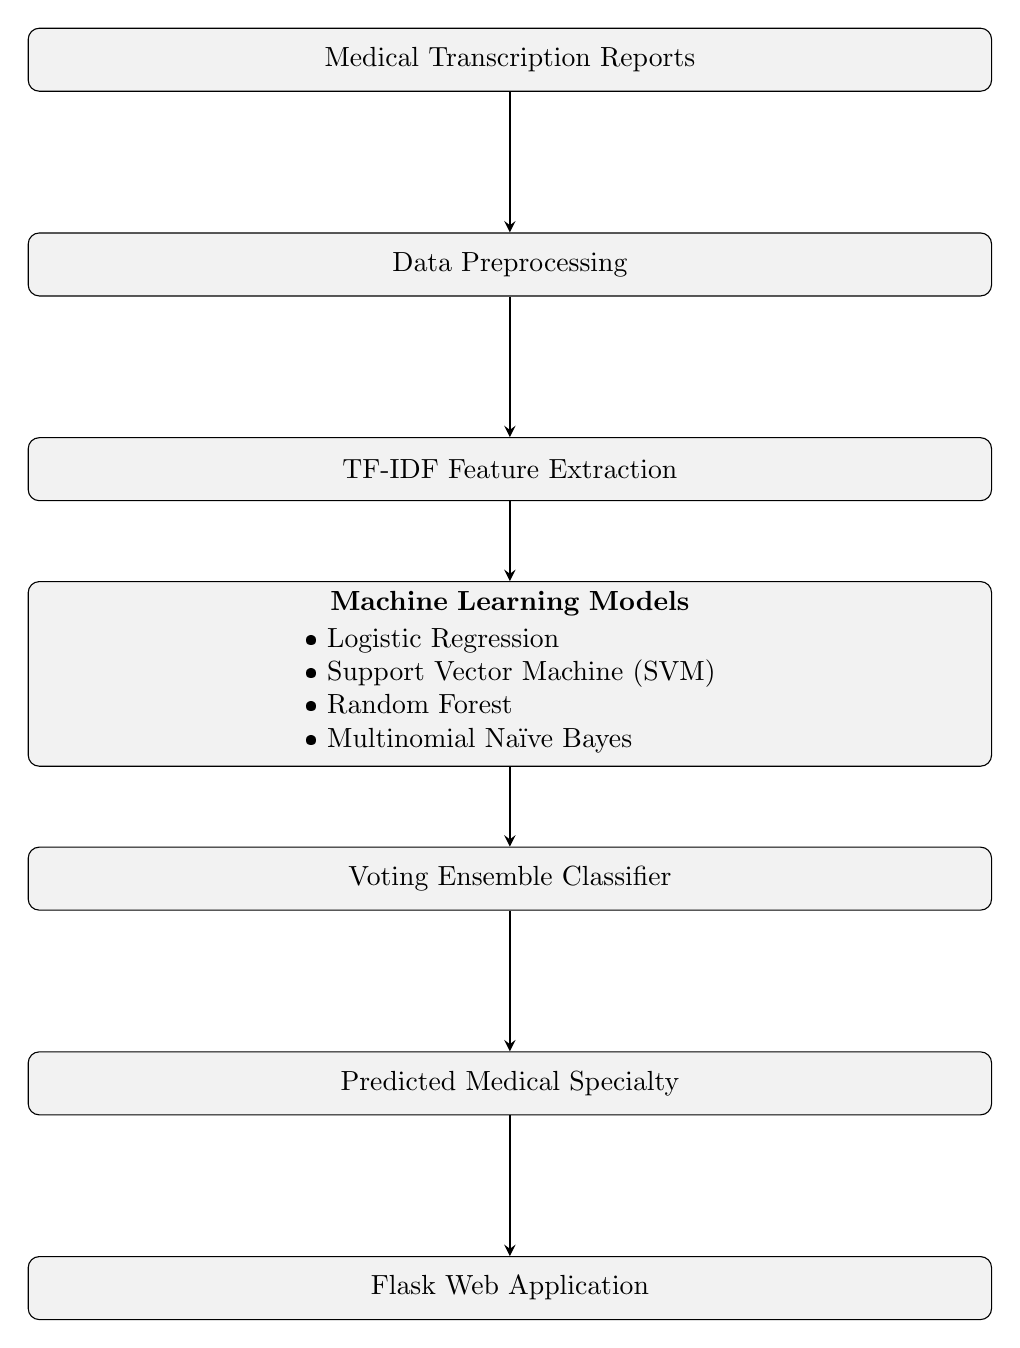
\begin{tikzpicture}[
    node distance=2.6cm,
    box/.style={rectangle, draw, rounded corners, text width=12cm, align=center, minimum height=0.8cm, fill=gray!10},
    arrow/.style={thick,->,>=stealth}
]

\node (data) [box] {Medical Transcription Reports};
\node (prep) [box, below of=data] {Data Preprocessing};
\node (tfidf) [box, below of=prep] {TF-IDF Feature Extraction};
\node (models) [box, below of=tfidf] {\textbf{Machine Learning Models} \\[0.5ex] \begin{tabular}{l} \textbullet~Logistic Regression \\ \textbullet~Support Vector Machine (SVM) \\ \textbullet~Random Forest \\ \textbullet~Multinomial Naïve Bayes \end{tabular}};
\node (ensemble) [box, below of=models] {Voting Ensemble Classifier};
\node (output) [box, below of=ensemble] {Predicted Medical Specialty};
\node (flask) [box, below of=output] {Flask Web Application};

\draw [arrow] (data) -- (prep);
\draw [arrow] (prep) -- (tfidf);
\draw [arrow] (tfidf) -- (models);
\draw [arrow] (models) -- (ensemble);
\draw [arrow] (ensemble) -- (output);
\draw [arrow] (output) -- (flask);

\end{tikzpicture}
\caption{Overall Workflow of the Proposed System}
\end{figure}

The complete system workflow follows a linear pipeline: Medical transcription data is ingested and rigorously cleaned through the NLP preprocessing stage. The standardized text is mathematically vectorized via TF-IDF into high-dimensional numerical features. These features are simultaneously evaluated by Logistic Regression, SVM, Random Forest, and Naïve Bayes algorithms. Their independent predictions are aggregated by the Voting Ensemble Classifier to produce the final, definitive medical specialty classification. This entire prediction engine is ultimately served via the Flask web interface for end-user interaction.

\par
\chapter{Expected Outcomes}
The proposed project is expected to successfully deliver a robust, automated classification engine encapsulated within a user-friendly Flask web application. The completed system will be capable of ingesting raw, unstructured medical transcription reports and accurately predicting their corresponding medical specialty in real-time, operating with computational efficiency.

The integration of this system is anticipated to yield expected benefits for healthcare document classification. By automating the categorization process, the system will reduce the necessity for manual document sorting. This will improve administrative efficiency, enhance the speed of data retrieval, and ensure that patient documents are consistently routed to the correct clinical departments. 

Academically and technologically, the expected contribution of this project is substantial. The project is expected to demonstrate the viability and accuracy of combining traditional NLP statistical techniques (TF-IDF) with aggregated Voting Ensemble architectures. The proposed system is expected to show that complex medical text classification can be successfully achieved efficiently, providing a scalable and highly interpretable alternative to computationally exorbitant deep learning frameworks.

\par
\chapter{Conclusion}
In conclusion, the manual classification of medical transcription reports is an administrative bottleneck in modern healthcare. This proposal outlines a computationally efficient automated solution utilizing Natural Language Processing and Ensemble Machine Learning. By systematically preprocessing clinical text, extracting TF-IDF features, and aggregating the predictive power of multiple algorithms into a Voting Ensemble Classifier, the proposed system is expected to provide accurate specialty categorizations. This approach is suitable for the problem as it balances predictive accuracy with interpretability and computational cost. In the subsequent phase, this methodology will be implemented in Python, evaluated, and deployed as a functional web application to demonstrate its practical utility in streamlining clinical informatics workflows. Ultimately, the successful deployment of this system is expected to reduce administrative burdens, enhance document routing, and improve overall operational efficiency within healthcare facilities. The immediate next phase of this project will focus entirely on the implementation, evaluation, and eventual real-world deployment of the proposed models.


\renewcommand\bibname{References}
\begin{thebibliography}{10}

\bibitem{Wang2023}
Y. Wang \textit{et al.}, ``Medical Text Classification Based on the Discriminative Pre-training Model and Prompt-Tuning,'' \textit{DIGITAL HEALTH}, vol. 9, 2023, doi: 10.1177/20552076231193213.

\bibitem{Almazaydeh2023}
L. Almazaydeh \textit{et al.}, ``Clinical Text Classification with Word Representation Features and Machine Learning Algorithms,'' \textit{International Journal of Online and Biomedical Engineering (iJOE)}, vol. 19, no. 4, 2023, doi: 10.3991/ijoe.v19i04.36099.

\bibitem{Zhang2023}
H. Zhang \textit{et al.}, ``Medical Specialty Classification Based on Semiadversarial Data Augmentation,'' \textit{Computational Intelligence and Neuroscience}, 2023, Art. no. 4919371, doi: 10.1155/2023/4919371.

\bibitem{Blanchard2022}
A. E. Blanchard \textit{et al.}, ``A Keyword-Enhanced Approach to Handle Class Imbalance in Clinical Text Classification,'' \textit{IEEE Journal of Biomedical and Health Informatics}, vol. 26, no. 6, pp. 2796--2803, 2022, doi: 10.1109/JBHI.2022.3141976.

\bibitem{Kesiku2022}
C. Y. Kesiku \textit{et al.}, ``Natural Language Processing Techniques for Text Classification of Biomedical Documents: A Systematic Review,'' \textit{Information}, vol. 13, 2022, Art. no. 499, doi: 10.3390/info13100499.

\bibitem{Mao2023}
C. Mao \textit{et al.}, ``Automatic Medical Specialty Classification Based on Patients' Description of Their Symptoms,'' \textit{BMC Medical Informatics and Decision Making}, vol. 23, 2023, Art. no. 15, doi: 10.1186/s12911-023-02105-7.

\end{thebibliography}

\end{document}
